\documentclass[presentation]{beamer}
%\documentclass[handout]{beamer}
\usetheme{Frankfurt}
\usecolortheme{seahorse}

\usepackage{amssymb}
\usepackage{amsmath}
\usepackage{graphicx}
\usepackage{subfig}
\usepackage{multicol}
\usepackage[font={footnotesize,it}]{caption}

\usepackage{tikz}
\usetikzlibrary{graphdrawing,graphs} 
\usegdlibrary{layered}
\usegdlibrary{force}
\usegdlibrary{trees}

\usepackage{hyperref}

\begin{document}

\title{Using Time Series Models for Defect Prediction in Software Release Planning}
\author{James Tunnell \\
Central Washington University \\
Computational Science Program}
\date{March 30, 2015}

\begin{frame}
\titlepage
\end{frame}

\begin{frame}
\small{
\frametitle{Outline}
\tableofcontents[hideallsubsections] 
}
\end{frame}

\section{Introduction}

\begin{frame}
\begin{center}
\Large{Introduction}
\end{center}
\end{frame}

\subsection{Release Planning}

\begin{frame}[t]
\frametitle{Release Planning Objectives}
\begin{itemize}
\item{Two primary objectives of software release planning are:
  \begin{itemize}
    \item{Improving functionality}
    \item{Maintaining quality}
  \end{itemize}}
  \item{Both of these objectives are constrained by limits on development time and cost.}
\end{itemize}
\end{frame}

\subsection{Quality Control}

\begin{frame}[t]
\frametitle{Quality Control}
\begin{itemize}
  \item{Software defects (bugs) are inevitable}
  \item{Sufficient time should be available to ensure good quality (by testing and bug-fixing)}
  \item{Otherwise, there is a risk of
    \begin{itemize}
    \item{Low quality (failure to meet objective)}
    \item{Schedule slip (failure to respect constraint)}
    \end{itemize}
  }
  \item{This quality control (QC) time can be allowed for by limiting the scope of work in the planned release}
\end{itemize}
\end{frame}

\begin{frame}[t]
\frametitle{Quality Control (cont'd)}
\begin{itemize}
  \item{To support release planning, QC time can be estimated}
  \item{Assumption: QC time depends (at least partly) on the number of software defects introduced}
  \item{Then, a basis for estimating QC time would be the predicted number of defects}
\end{itemize}
\end{frame}

\subsection{Defect Prediction}

\begin{frame}[t]
\frametitle{Defect Prediction}
\begin{itemize}
  \item{Approaches to defect prediction tend to focus on either
    \begin{itemize}
    \item{Code analysis
      \begin{itemize}
      \item{Lines of code}
      \item{Number of decisions}
      \item{Code churn}
      \end{itemize}
    }
    \item{Historical information
      \begin{itemize}
      \item{Regression analysis}
      \item{Time series modeling}
	  \end{itemize}
	}
    \end{itemize}
  }
  \item{A multivariate time series model with exogenous inputs was chosen}
\end{itemize}
\end{frame}

\subsection{Related Work: Using Code Analysis}

\begin{frame}[t]
\frametitle{Defect Prediction using Code Analysis}
\begin{itemize}
\item{Approaches using code analysis:
  \begin{itemize}
  \item{Akiyama used lines of code (LOC), number of decisions, and the number of subroutine calls \cite{1971_akiyama}}
  \item{Gafney also used LOC \cite{1984_gaffney_estimating}}
  \item{Henry and Kafura use information taken from design documents \cite{1984_henry_evaluation}}
  \item{Nagappan and Ball use relative code churn (lines modified) \cite{2005_nagappan_codechurn}}
  \end{itemize}
}
\item{These approaches all depend on specific design or implementation information}
\item{This information is not available at the release planning stage}
\end{itemize}
\end{frame}

\subsection{Related Work: Using Historical Information}

\begin{frame}[t]
\frametitle{Defect Prediction using Historical Information}
\begin{itemize}
\item{Approaches using historical information:
  \begin{itemize}
  \item{Li et al. extrapolate parameters of a regression model \cite{2004_li_emperical_eval}}
  \item{Singh et al. use an ARIMA time series model \cite{2010_singh_predicting}}
  \end{itemize}
}
\item{Both approaches are non-specific to design or implementation}
\item{However, neither approach is explanatory}
\end{itemize}
\end{frame}

\section{Motivation}

\begin{frame}
\begin{center}
\Large{Motivation}
\end{center}
\end{frame}

\subsection{Release Plan Optimization}

\begin{frame}[t]
\frametitle{Release Plan Optimization}
\begin{itemize}
  \item{A release plan is formed by selecting features and improvements to work on}
  \item{Release plans can be compared by the expected revenue they will generate}
  \item{This optimization problem is posed as The Next Release Problem (NRP)}
\end{itemize}
\end{frame}

\begin{frame}[t]
\frametitle{Release Plan Optimization (cont'd)}
\begin{itemize}
  \item{The NRP is an abstract optimization problem}
  \item{In practice, QC time should be considered to ensure constraints are respected}
  \item{With the help of a defect prediction model, QC time can be estimated}
  \item{In this context, release plans are being compared}
  \item{For a defect prediction model to be useful, it should depend in some way on the basic elements of the release plan (planned new features and improvements)}
\end{itemize}
\end{frame}

\subsection{Explanatory Model}

\begin{frame}[t]
\frametitle{Explanatory Model}
\begin{itemize}
\item{Assumption: the number of defects in the future depends on more than just the number of defects in the past}
\item{A defect prediction model that depends only on previous numbers of defects is not explanatory}
\item{Such a non-explanatory model would always predict the same number of defects}
\end{itemize}

\begin{figure}[htbp]
\begin{center}
\tikz[nodes={text height=1em, text depth=.2em, draw=black!20, thick, fill=white, font=\small}, rounded corners, semithick]
  \graph[layered layout, level distance = 1cm, sibling sep = 1em]{
    "Release Plan 1" -> "Explanatory Model";
    "Release Plan 2" -> "Explanatory Model";
    "...." -> "Explanatory Model";
    "Release Plan N" -> "Explanatory Model";
    "Explanatory Model" -> "Predicted Defects";
  };
\caption{A non-explanatory model.}
\end{center}
\end{figure}
\end{frame}


\begin{frame}[t]
\frametitle{Explanatory Model (cont'd)}
\begin{itemize}
\item{A model could also depend on the key factors of a release plan}
\item{This would be an explanatory model structure}
\item{Such a model can potentially predict a different number of defects for every release plan}
\end{itemize}

\begin{figure}[htbp]
\begin{center}
\tikz[nodes={text height=1em, text depth=.2em, draw=black!20, thick, fill=white, font=\small}, rounded corners, semithick]
  \graph[layered layout, level distance = 1cm, sibling sep = 1em]{
    "Release Plan 1" -> "Explanatory Model";
    "Release Plan 2" -> "Explanatory Model";
    "...." -> "Explanatory Model";
    "Release Plan N" -> "Explanatory Model";
    "Explanatory Model" -> "Predicted Defects 1";
    "Explanatory Model" -> "Predicted Defects 2";
    "Explanatory Model" -> "...";
    "Explanatory Model" -> "Predicted Defects N";
  };
\caption{An explanatory model.}
\end{center}
\end{figure}
\end{frame}

\section{Time Series}

\begin{frame}
\begin{center}
\Large{Time Series Modeling}
\end{center}
\end{frame}


\subsection{Time Series}

\begin{frame}[t]
\frametitle{Time Series }
\begin{itemize}
\item{A time series is a collection of observations that occur in order}
\item{The process underlying a time series is assumed to be stochastic (non-deterministic)}
\item{Each observation might depend on one or more previous observations}
\item{This dependence is termed autocorrelation}
\end{itemize}
\end{frame}

\subsection{Autoregressive Models}

\begin{frame}[t]
\frametitle{Autoregressive Models}
\begin{itemize}
\item{A basic autoregressive (AR) model is a linear combination of previous values}
\item{A white noise term accounts for stochastic fluctuation}
\item{An $AR(p)$ model for predicting a value X at time t is
\begin{equation}
X_t=c+\sum_{i=1}^{p}{\phi_t X_{t-1}+\epsilon_t}
\end{equation}
where $\phi_1, \phi_2, ..., \phi_p$ are the $p$ parameters, $c$ is a constant, and $\epsilon_t$ is the white noise term}
\end{itemize}
\end{frame}

\begin{frame}[t]
\frametitle{Autoregressive Models (cont'd)}
\begin{itemize}
\item{Extending the AR model to be multivariate results in a Vector AR (VAR) model}
\item{This model can support time series for defect count, improvements, and new features}
\end{itemize}
\end{frame}

\subsection{Endogeneity and Exogeneity}

\begin{frame}[t]
\frametitle{Endogeneity and Exogeneity}
\begin{itemize}
\item{Under a VAR model, the behavior of each time series is explained by both
its own past values and the past values of the other time series}
\item{This makes the variables endogenous}
\item{An alternative is that a time series is only used to explain other time series}
\item{This type of explanatory variable is called exogenous, and could be considered an input}
\item{Exogenouse variables are not explained by the model}
\end{itemize}
\end{frame}

\begin{frame}[t]
\frametitle{Endogeneity and Exogeneity (cont'd)}
\begin{itemize}
\item{The desired model does not need to explain features and improvements}
\item{Instead, these are used to explain defects}
\item{Planned features and improvements can be made exogenous}
\item{By also considering exogenous variables, a VAR model would become a
VARX model}
\end{itemize}
\end{frame}

\subsection{Stationarity and Trends}

\begin{frame}[t]
\frametitle{Stationarity}
\begin{itemize}
\item{A stationary time series has time-invariant statistics}
\item{The time series models so far require time series to be stationary}
\item{Differencing a non-stationary series may produce a stationary series}
\item{Stationary can be determined by testing for trends}
\end{itemize}
\end{frame}

\begin{frame}[t]
\frametitle{Deterministic Trends}
\footnotesize{
\begin{itemize}
\item{A time series with a deterministic trend has a non-constant mean}
\item{The time series movements will generally follow the deterministic function}
\item{Fluctuations above or below this function are non-permanent}
\item{Such a time series is said to be stationary around a deterministic trend}
\end{itemize}
}
\begin{figure}[htbp]
\begin{center}
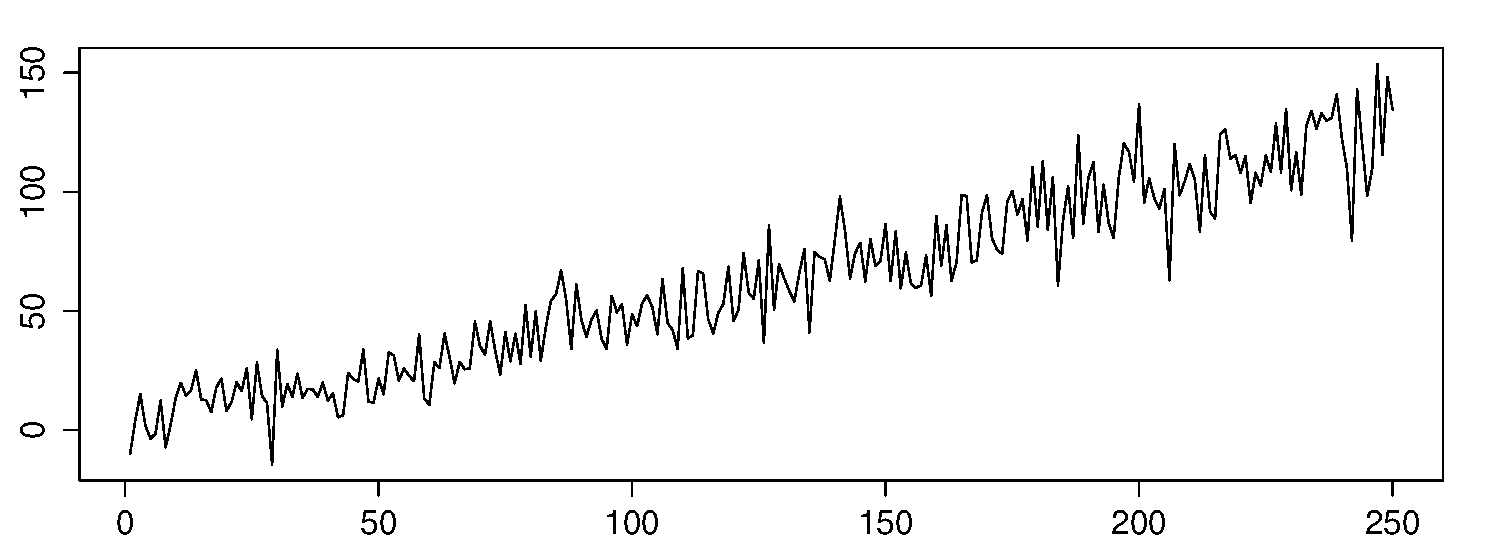
\includegraphics[width=\textwidth]{assets/deterministic_trend.eps}
\caption{Time series with a deterministic trend.}
\end{center}
\end{figure}
\end{frame}


\begin{frame}[t]
\frametitle{Stochastic Trends}
\footnotesize{
\begin{itemize}
\item{A stochastic trend shows permanent effects due to random variations}
\item{A series with stochastic trend will not necessarily fluctuate only close to the area of a deterministic function}
\item{A time series with stochastic trend is non-stationary}
\item{Differencing can be used to remove a stochastic trend}
\end{itemize}
}
\vspace{-.2cm}
\begin{figure}[htbp]
\begin{center}
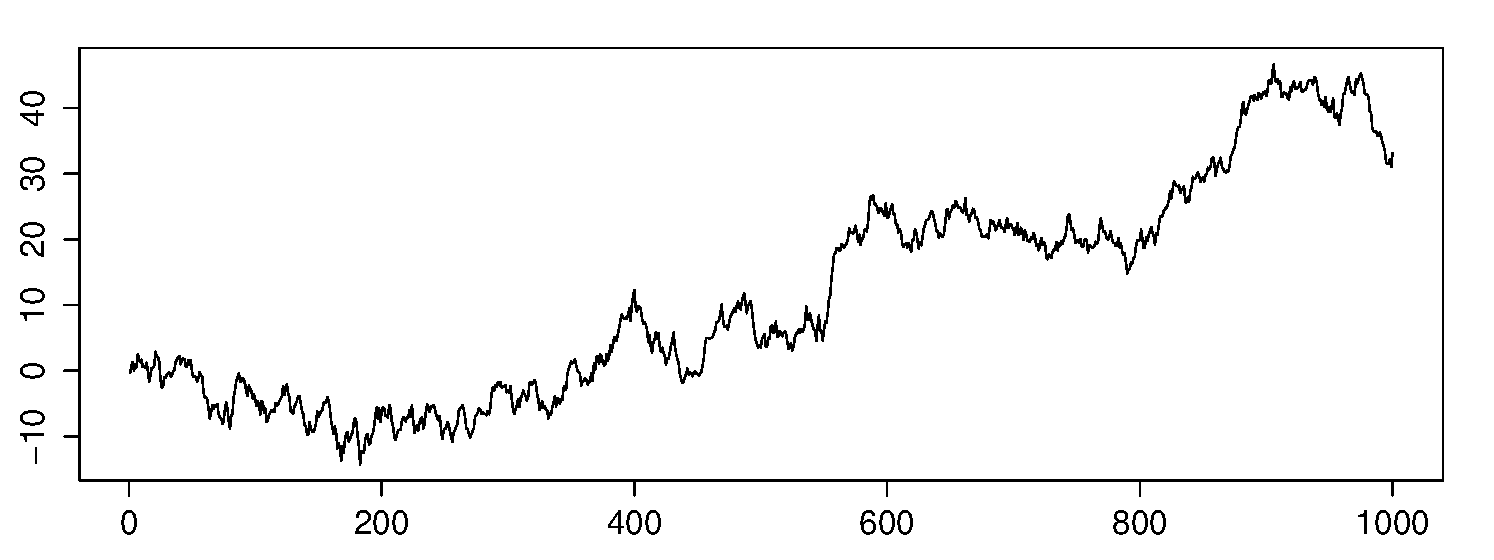
\includegraphics[width=\textwidth]{assets/stochastic_trend.eps}
\caption{Time series with a stochastic trend.}
\end{center}
\end{figure}
\end{frame}

\subsection{Stationarity Testing}

\begin{frame}[t]
\frametitle{Stationarity Testing}
\footnotesize{
\begin{itemize}
\item{A pure AR model of a time series with stochastic trend contains a unit root \cite{franses1998time}}
\item{Testing for the presence of a unit root can therefore be used to test for non-stationarity}
\item{A unit-root test starts with the null hypothesis that an AR model has a unit root}
\item{The alternative hypothesis is that an AR model of the time series does not have a unit root}
\item{Next, a test statistic is measured}
\item{If the test statistic is below the chosen significance level, the null hypothesis is rejected}
\item{Rejecting the null hypothesis provides reason to accept the alternative hypothesis}
\item{The Augmented Dickey Fuller (ADF) test is commonly used for unit root testing}
\end{itemize}
}
\end{frame}

\begin{frame}[t]
\frametitle{Stationarity Testing (cont'd)}
\footnotesize{
\begin{itemize}
\item{On the other hand is a stationarity test}
\item{This test starts with the null hypothesis that a time series is stationary around a deterministic trend}
\item{If the test statistic is above some significance level, this shows that the null hypothesis can be accepted}
\item{Then the time series should be considered stationary}
\item{The Kwiatkowski-Phillips-Schmidt-Shin (KPSS) test can be applied for testing stationarity.}
\end{itemize}
}
\end{frame}

\section{Modeling Methodology}

\begin{frame}
\begin{center}
\Large{Modeling Methodology}
\end{center}
\end{frame}

\subsection{Overview}

\begin{frame}[t]
\frametitle{Time Series Modeling Methodology}
\begin{itemize}
\item{Time series modeling methodology typically involves
  \begin{enumerate}
  \item{Specification}
  \item{Estimation}
  \item{Diagnostic Checking}
  \item{Selection}
  \end{enumerate}}
\end{itemize}
\end{frame}

\subsection{Specification \& Estimation}

\begin{frame}[t]
\frametitle{Specification \& Estimation}
\begin{itemize}
\item{A $VARX(p)$ model is specified by choosing an order $p$}
\item{Model order is the number of autoregressive terms}
\item{This affects the number of parameters included in the model}
\item{To avoid having too many parameters relative to the number of observations, we use
  \begin{equation}
  p_{max} = \left \lfloor \frac{n}{m K_{min}} \right \rfloor
  \end{equation}
  
  \begin{itemize}
    \item{$n$ is the number of time samples}
    \item{$m$ is the number of time series}
    \item{$K_{min}$ is the minimum acceptable ratio of observations to parameters}
  \end{itemize}
  }
\item{Models parameters are estimated for orders $1, 2,..., p_{max}$}
\end{itemize}
\end{frame}


\subsection{Diagnostic Checking}

\begin{frame}[t]
\frametitle{Diagnostic Checking}
\begin{itemize}
\item{Diagnostics can tell if a model should be rejected}
\item{First diagnostic is for stability
  \begin{itemize}
  \item{AR model can have infinite impulse response}
  \item{To be stable, the roots of the characteristic equation must lie outside the unit circle \cite[p. 56]{box_jenkins_reinsel_2008}}
  \item{Equivalently, the inverse of the roots must lie inside the unit circle}
  \end{itemize}
}
\item{Next diagnostic is residual autocorrelation
  \begin{itemize}
    \item{Model residuals should be indistinguishable from white noise}
    \item{White noise is uncorrelated (no autocorrelation)}
    \item{Ljung-Box test forms a statistic from the autocorrelation of the residuals}
  \end{itemize}
}
\end{itemize}
\end{frame}

\subsection{Model Selection}

\begin{frame}[t]
\frametitle{Model Selection}
\begin{itemize}
\item{Model selection criteria are used to compare models according to their fit}
\item{penalties for residual error and the number of parameters}
\item{Some common selection criteria
  \begin{itemize}
  \item{Akaike Information Criterion (AIC)}
  \item{AIC with correction (AICc)}
  \item{Bayesian Information Criterion (BIC)}
  \end{itemize}
}
\item{Parameter penalty is more severe for BIC and AICC than for AIC \cite{bisgaard2011time}}
\item{Prefer AIC, since the number of parameters is already limited in the specification step}
\end{itemize}
\end{frame}

\section{Data Methodology}

\begin{frame}
\begin{center}
\Large{Data Methodology}
\end{center}
\end{frame}

\note{In this section, the data source and data collection method are detailed. Then, the method of preparing data for the modeling phase is presented.}

\subsection{Data Source}

\begin{frame}[t]
\frametitle{Data source}
\begin{itemize}
\item{Data for time series modeling will be derived from project historical data}
\item{This historical data can be found in the project issue tracking system (ITS)}
\item{The issues in an ITS can be bugs, features, improvements, etc.}
\item{The \textit{MongoDB} software project was selected to try out the modeling methodology
\begin{itemize}
\item{The project has been actively developed since 2009}
\item{Data from versions 0.9.3 through 3.0.0-rc6 are used}
\item{This dataset contained $7042$ issues}
\end{itemize}
}
\end{itemize}
\end{frame}

\subsection{Data Collection}

\begin{frame}[t]
\frametitle{Data Collection}
\begin{itemize}
\item{\textit{MongoDB} uses \textit{JIRA} for issue tracking and project management}
\item{Issue data was exported from the project's JIRA web interface as XML data}
\item{Issue data was extracted from the XML, and the following fields were kept:
  \begin{itemize}
  \item{Creation date}\item{Resolution date}\item{Type}\item{Priority}
  \end{itemize}
}
\end{itemize}
\end{frame}

\subsection{Data Cleansing}

\begin{frame}[t]
\frametitle{Data Cleansing}
\begin{itemize}
\item{Not all of the data was preserved for modeling}
\item{No-change issues
  \begin{itemize}
  \item{Only issues with resolution \textit{fixed}, \textit{complete}, or \textit{done} were be kept}
  \item{Other issues did not result in any change, and were not included}  
  \end{itemize}
}
\item{Orphan sub-tasks
  \begin{itemize}
  \item{Issues that are sub-tasks are first converted to be the same type as the parent issue}
  \item{Sub-tasks whose parent issue is not in the dataset are considered orphans, and discarded}
  \item{Orphan sub-tasks can not be identified as improvement or new feature}
  \item{$20$ ($0.28\%$) orphaned sub-tasks were in the dataset}
  \end{itemize}
}
\end{itemize}
\end{frame}

\subsection{Data Preparation}

\begin{frame}[t]
\frametitle{Data Sampling}
\begin{itemize}
\item{The dataset was operated on to prepare it for time series modeling}
\item{First, data was sampled at regular intervals, measuring
  \begin{itemize}
  \item{Number of bugs created}
  \item{Number of improvements resolved}
  \item{Number of new features resolved}
  \end{itemize}
}
\item{A 7-day sampling period was used}
\end{itemize}
\end{frame}

\begin{frame}[t]
\frametitle{Data Sampling (cont'd)}

\tiny{
  \begin{figure}[htbp]
  \begin{center}
  \begin{tikzpicture}[scale=.4]
    \tikzstyle{every node}=[font=\tiny]
    \node (bb) at (-2.5,2) [draw] {|Bug|};
    \node (n) at (-2.5,1) [draw] {|New Feature|};
    \node (ii) at (-2.5,0) [draw] {|Improvement|};
    \node (bbbb) at (-1,-1) [draw] {|Bug|};
    \node (i) at (0,-2) [draw] {|Improvement|};
    \node (bbbbb) at (1.4,-3) [draw] {|Bug|};
    \draw[dashed] (-3,3) -- (-3,-4);
    \draw[dashed] (0,3) -- (0,-4);
    \draw[dashed] (3,3) -- (3,-4);
    \draw (-4.5,3.5) node {Period 1};
    \draw (-1.5,3.5) node {Period 2};
    \draw (1.5,3.5) node {Period 3};
    \draw (4.5,3.5) node {...};
  \end{tikzpicture}
  \caption{Sampling example issue data.}
  \end{center}
  \end{figure}

  \vspace{.2cm}
  \begin{table}[htbp]
  \centering
  \begin{tabular}{ c | c | c | c }
  \hline
  Period & Improvements & New Features & Bugs \\
  ~& Resolved & Resolved & Created \\
  \hline
  1 & 0 & 0 & 1 \\
  2 & 1 & 1 & 1 \\
  3 & 1 & 0 & 1 \\
  \hline
  \end{tabular}
  \caption{Results of sampling example issues.}
  \end{table}
}
\end{frame}

\begin{frame}[t]
\frametitle{Establishing Stationarity}
\begin{itemize}
\item{Establish stationarity by testing
  \begin{itemize}
  \item{ADF unit root test}
  \item{KPSS stationariy test}
  \end{itemize}}
\item{If test results agree, then no differencing is necessary}
\item{Otherwise, difference data and retest}
\end{itemize}
\end{frame}

\begin{frame}[t]
\frametitle{Time Windowing}
\begin{itemize}
\item{Assumption: the software development process underlying a given project might change over time}
\item{The VARX model does not accommodate a changing process}
\item{To account for a changing process, data will be time windowed}
\item{Data will be used for modeling only if it occurs within the time window}
\item{This should limit the amount of process change the model is exposed to}
\end{itemize}
\end{frame}

\section{Results}

\begin{frame}
\begin{center}
\Large{Results}
\end{center}
\end{frame}

\subsection{Data Methodology}

\begin{frame}[t]
\frametitle{\textit{MongoDB} Time Series Data}
Time series data was obtained by sampling the \textit{MongoDB} dataset with a 7-day sample period
\begin{figure}[htbp]
\begin{center}
\includegraphics[height=.6\textheight]{assets/time_series.eps}
\caption{\textit{MongoDB} time series data}
\end{center}
\end{figure}
\end{frame}

\begin{frame}[t]
\frametitle{Stationarity \& Differencing}
\footnotesize{
\begin{itemize}
\item{At first, ADF and KPSS test results disagreed}
\item{After differencing, test results agreed}
\end{itemize}
}
\vspace{-.5cm}
\begin{figure}[htbp]
\begin{center}
\includegraphics[height=.6\textheight]{assets/time_series_diff.eps}
\caption{\textit{MongoDB} time series data after differencing}
\end{center}
\end{figure}
\end{frame}

\begin{frame}[t]
\frametitle{Time Windowing}
\begin{itemize}
\item{A 78-week time window (approximately 18 months) was chosen}
\item{Three of these windowed periods, non-overlapping, were used for modeling}
\item{Since the data is being differenced, the first sample (week) is skipped}
\item{These windowed periods are denoted $W_{2-79}$, $W_{80-157}$, and $W_{158-235}$}
\item{Modeling methodology is applied to each}
\end{itemize}
\end{frame}

\subsection{Modeling Methodology}

\begin{frame}[t]
\frametitle{Model Specification, Estimation, and Diagnostic Checking}
\begin{itemize}
\item{Using $K_{min} = 4$, maximum model order is obtained by
\begin{equation}
p_{max} = \left \lfloor \frac{78}{(3)(4)} \right \rfloor = \lfloor 6.5 \rfloor = 6
\end{equation}
}
\item{Models of order $1$ through $p_{max}=6$ were estimated for diagnostic checking}
\item{All models were found to be stable}
\item{Several model orders were found to be inadequate by the Ljung-Box test:
  \begin{itemize}
  \item{Orders 1-2 for period $W_{2-79}$}
  \item{Order 5 for period $W_{158-235}$}
  \end{itemize}
}
\end{itemize}
\end{frame}

\begin{frame}[t]
\frametitle{Model Selection}
\begin{itemize}
\item{Models found to be stable and not inadequate were considered for selection}
\item{A different model was selected for each windowed period}
\item{Lower AIC score is better}
\end{itemize}
\footnotesize{
\begin{table}[htbp]
  \centering
  \begin{tabular}{ c | r | r | r }
    ~ & \multicolumn{3}{|c}{AIC score} \\
    Model order & $W_{2-79}$ & $W_{80-157}$ & $W_{158-235}$ \\
    \hline
    1 & N/A & \textbf{429.8} & \textbf{477.9} \\
    2 & N/A & 439.3 & 482.4 \\
    3 & 400.8 & 440.9 & 489.7 \\
    4 & \textbf{400.3} & 450.2 & 499.9 \\ 
    5 & 404.0 & 456.7 & N/A \\
    6 & 414.9 & 461.7 & 508.8 \\
    \hline
  \end{tabular}
\caption{Results of model selection, using AIC score to compare models of different order.}
\end{table}
}
\end{frame}


\begin{frame}[t]
\frametitle{One-step Predictions}
\small{The fit for each selected model is demonstrated by plotting one-step predictions along with actual values.}

\begin{figure}[htbp]
\centering
\vspace{-.25in}
\subfloat{
\includegraphics[width=.65\textwidth]{assets/one-step_predictions_2-79.eps}
}\\
\vspace{-.6in}
\subfloat{
\includegraphics[width=.65\textwidth]{assets/one-step_predictions_80-157.eps}
}\\
\vspace{-.6in}
\subfloat{
\includegraphics[width=.65\textwidth]{assets/one-step_predictions_158-235.eps}
}%
\caption{Actual values (solid) vs. one-step predictions (dotted), for each model selected by AIC score.}
\end{figure}
\end{frame}


\subsection{Forecasting}

\begin{frame}[t]
\frametitle{Forecasting Results}
\begin{itemize}
\item{A range of hypothetical future values for improvements and new features were used to make defect predictions}
\item{This simulates the use of defect prediction for release planning}
\item{Single-step, out-of-sample forecast}
\item{Inputs were differenced, and difference was removed from output}
\item{Results include 75\% and 90\% confidence intervals}
\item{Forecast results are shown only for the first time window, $W_{2-79}$}
\end{itemize}
\end{frame}

\begin{frame}[t]{Forecasting Results (cont'd)}
\footnotesize{
\begin{itemize}
\item{The actual number of improvements and features was 4 and 0}
\item{Actual number of bugs was 18}
\item{For the actual input values, the 90\% confidence interval does not include 18}
\end{itemize}

\vspace{-.5cm}
\begin{table}[htbp]
  \centering
\caption{Forecasting at the end of the first time window, $W_{2-79}$.}
  \begin{tabular}{ c | c | c | c | c | c | c }
    Improvements & Features & 90\% low & 75\% low & Mean & 75\% high & 90\% high \\
    \hline
2 & 0 & 5.61 & 6.72 & 9.31 & 11.89 & 13.00 \\
2 & 1 & 5.54 & 6.66 & 9.24 & 11.82 & 12.93 \\
2 & 2 & 5.48 & 6.59 & 9.17 & 11.75 & 12.86 \\
2 & 3 & 5.41 & 6.52 & 9.1 & 11.69 & 12.8 \\
4 & 0 & 6.4 & 7.51 & 10.09 & 12.68 & 13.79 \\
4 & 1 & 6.33 & 7.44 & 10.03 & 12.61 & 13.72 \\
4 & 2 & 6.27 & 7.38 & 9.96 & 12.54 & 13.65 \\
4 & 3 & 6.2 & 7.31 & 9.89 & 12.48 & 13.59 \\
    \hline
  \end{tabular}
\end{table}
}
\end{frame}


\begin{frame}[t]{Forecasting Results (cont'd)}
\begin{itemize}
\item{Low accuracy for the predictions is concerning}
\item{For the next window, $W_{80−157}$, the actual number of future bugs was 17}
\item{This was inside the 90\% confidence interval, which spanned from 13.38 to 18.00}
\item{How useful is the VARX model in general, considering these conflicting results?}
\item{To find out, a sliding 78-week window was used}
\item{The sliding window started at the first sample period, and was shifted by one sample period after modeling}
\item{Only the actual number of improvements and features were used in this forecasting}
\end{itemize}
\end{frame}

\begin{frame}[t]{Sliding Window Results}
\footnotesize{
\begin{itemize}
\item{Errors between the mean forecasted and actual number of bugs is shown as a histogram}
\item{The histogram appears to be normally distributed (good)}
\item{The variability is quite large (bad)}
\item{The actual number of bugs was inside the 90\% confidence interval for 23.87\% of the sliding window ranges}
\end{itemize}
\vspace{-.5cm}
\begin{figure}[htbp]
\begin{center}
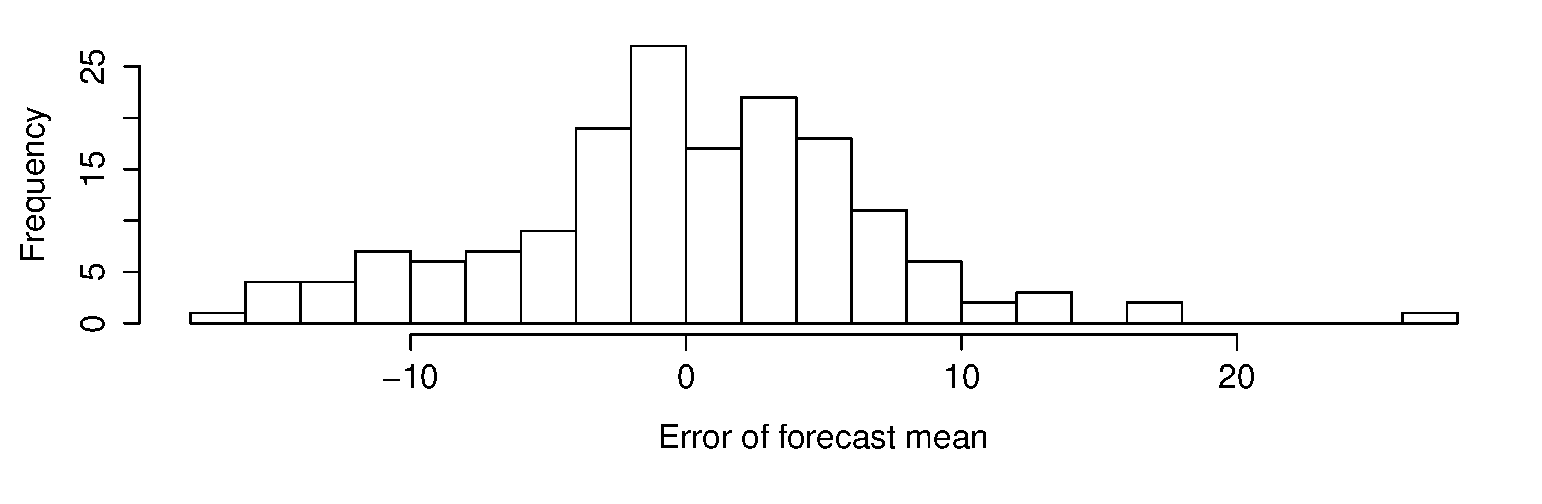
\includegraphics[width=.9\textwidth]{assets/forecast_errors.eps}
\caption{Histogram of errors in forecast mean obtained using a 78-week sliding window.}
\end{center}
\end{figure}
}
\end{frame}


\section{Conclusions}

\begin{frame}
\begin{center}
\Large{Conclusion \& Future Work}
\end{center}
\end{frame}

\subsection{Conclusions}

\begin{frame}[t]{Conclusions}
\footnotesize{
\begin{itemize}
\item{The VARX modeling methodology was successfully applied to the time series data collected from the \textit{MongoDB} project}
\item{Models were created for each of three time windows}
\item{A model was selected for each window}
\item{Forecast results using the models were inconclusive}
\item{A better picture of the prediction performance was obtained using a sliding window}
\item{This resulted in a normally distributed error in the mean forecasted values}
\item{A low proportion (23.87\%) of the sliding window ranges included the actual number of bugs in the 90\% confidence interval}
\item{These results may indicate that a VARX model will not be useful to make predictions for the the MongoDB dataset}
\end{itemize}
}
\end{frame}

\subsection{Future Work}

\begin{frame}{Future Work}
Having applied the VARX time series model to one project dataset, a next step is to apply the methodology to other software project data sets, such as \textit{Eclipse} or \textit{Mozilla}, to more conclusively determine the model's usefulness.
\end{frame}

\section{References}

\begin{frame}[allowframebreaks]{References}
\begin{center}
\bibliography{references}
\bibliographystyle{abbrv}
\end{center}
\end{frame}

\end{document}
